% !TEX program = xelatex
\documentclass[11pt]{article}

\usepackage{fontspec}
\usepackage{xeCJK}
\usepackage{graphicx}
\usepackage[a4paper,top=0.65cm,bottom=0.75cm,left=1.25cm,right=1.25cm,nohead,nofoot]{geometry}
\usepackage{xcolor}
\usepackage{fontawesome}
\usepackage{titlesec}
\usepackage{enumitem}
\usepackage{hyperref}
\usepackage{tabularx}

\setlength{\parindent}{0pt}
\setmainfont{TeX Gyre Termes}
\setCJKmainfont{SimSun}
\setCJKsansfont{SimHei}
\setlist[itemize]{leftmargin=1.35em,itemsep=0.08em,topsep=0.18em,parsep=0em,partopsep=0em}
\definecolor{darkgreen}{RGB}{0,100,0}
\hypersetup{colorlinks=true,urlcolor=darkgreen,linkcolor=darkgreen,unicode=true}

\titleformat{\section}{\large\bfseries\raggedright}{}{0em}{}[\vspace{-0.35em}\titlerule]
\titlespacing*{\section}{0pt}{0.55em}{0.28em}
\titleformat{\subsection}{\normalsize\bfseries\raggedright}{}{0em}{}
\titlespacing*{\subsection}{0pt}{0.25em}{0.05em}
\newcommand{\datedsubsection}[2]{\subsection{#1 \hfill \normalfont #2}}
\newcommand{\tech}[1]{\textcolor{gray!85}{\small #1}}

\begin{document}
\pagenumbering{gobble}
\vspace*{-8pt}

\begin{tabularx}{\textwidth}{@{}X r@{}}
  \begin{minipage}[t]{0.78\textwidth}
    \centering
    {\LARGE\bfseries 张建}\\[3pt]
    {\normalsize 求职意向：AI 全栈开发}\\[2pt]
    \faEnvelope \href{mailto:m202473806@hust.edu.cn}{m202473806@hust.edu.cn}
    \quad \faPhone 15237776378\\[2pt]
    \faGlobe \href{https://husterzj.info/}{husterzj.info}
    \quad \faCodeFork \href{https://gitee.com/husterzj/spacetaskscheduler}{Gitee 项目仓库}
  \end{minipage}
  &
  \begin{minipage}[t]{0.15\textwidth}
    \raggedleft\vspace{-7pt}
    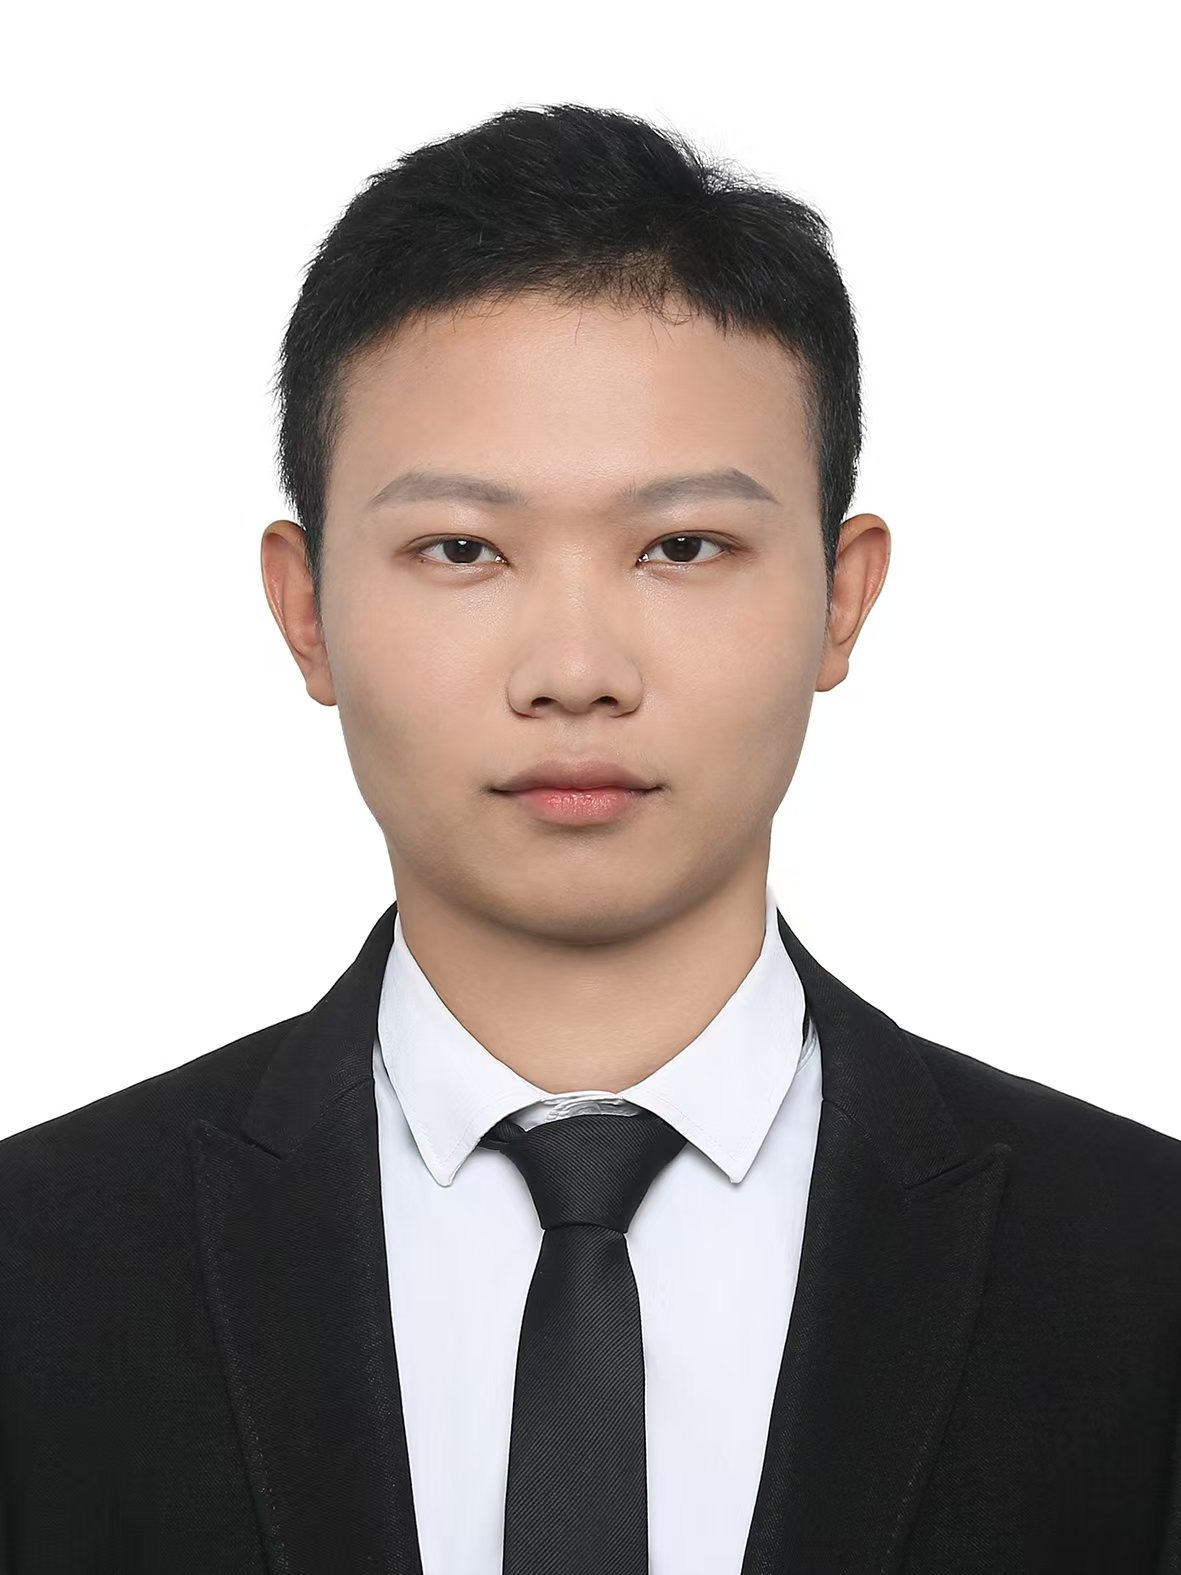
\includegraphics[width=0.83in]{zj.jpg}
  \end{minipage}
\end{tabularx}
\vspace{-5pt}

\section{\faCog 专业技能}
\begin{itemize}
  \item \textbf{产品与交付：}具备需求调研、竞品分析、业务建模、流程图与产品文档整理经验，参与功能测试、问题排查与方案复盘，能够从业务问题推进至系统实现和部署。
  \item \textbf{全栈开发：}熟悉 Python、FastAPI、Vue3、TypeScript、Pinia、MySQL/Supabase；具备 RESTful 接口、结构化数据协议、前后端联调、Git 与 Linux/Nginx 部署经验。
  \item \textbf{AI 应用：}了解 LLM Agent、Tool Use、MCP、Embedding 与向量检索；日常使用 Claude Code、Codex 等 AI 编码工具，具备低代码平台及 AI 工具链实践经验。
\end{itemize}

\section{\faGraduationCap 教育经历}
\datedsubsection{华中科技大学｜智能科学与技术｜学术型硕士}{2024.09 -- 2027.06（预计）}
人工智能与自动化学院；2024--2025 学年一等硕士学业奖学金
\datedsubsection{华中科技大学｜自动化｜工学学士}{2019.09 -- 2024.06}
本科加权成绩 88.1，GPA 3.83；2022 年排名 16/187；推免攻读硕士研究生

\section{\faBriefcase 实习经历}
\datedsubsection{武汉归心科技有限公司｜全栈开发工程师}{2026.06 -- 至今}
\tech{FastAPI · Supabase · Embedding · 向量检索 · AI 工具链}
\begin{itemize}
  \item 参与 AI 招聘与人才认证平台研发，梳理业务模块及 Epic/Story 依赖，推进 Story 2.1--2.3 的主要开发、手动测试、缺陷复测与结果同步。
  \item 排查企业端人才搜索异常，围绕 embedding 模型、向量维度、pgvector、数据覆盖率与评分日志定位问题，完成 embedding 服务切换及维度匹配调整。
  \item 通过 Supabase REST API 分析表结构与业务数据链路，形成数据库结构及修改建议；完成 BMad V4 至 V6 迁移相关文档重构和新人开发指南。
  \item 调研 Mercor、Juicebox、dinq 等 AI 招聘产品的功能、技术路线和商业模式，并参与“认证+简历”等产品方向讨论；修复生产环境 FastAPI 文档公网暴露问题。
\end{itemize}

\section{\faCode 项目经历}
\datedsubsection{航天器任务调度原型系统｜国自然重点项目相关}{2024.05 -- 2025.10}
\tech{Python · FastAPI · Vue3 · TypeScript · Pinia · Java · Nginx}
\begin{itemize}
  \item 参与真实航天任务规划场景的需求梳理与业务建模，将资源、任务、约束、算法配置和结果整理为可配置的 Web 原型系统，开发规划包、主视图、报告与日志等模块。
  \item 设计并实现“用户配置—数据转换—约束预处理—算法执行—结果解析—甘特图展示”链路；以标准化 JSON/CSV 协议将 Java 启发式算法接入 FastAPI 服务。
  \item 完成前后端联调与 Linux/Nginx 部署，形成可访问的\href{https://astroscheduler.cn/}{演示系统}和\href{https://gitee.com/husterzj/spacetaskscheduler}{开源仓库}，支持任务与资源双视角结果展示。
\end{itemize}

\datedsubsection{智慧校园一体化服务学工平台｜中国软件杯队长}{2023.08}
\tech{金蝶云苍穹 · 低代码 · 产品方案 · 数据分析}
\begin{itemize}
  \item 面向学生、教师、辅导员等角色梳理学工痛点，参与设计 PC 与移动端一体化方案，覆盖迎新、宿舍、资助、奖惩和学习管理等模块。
  \item 参与页面建模、业务流、权限、插件与轻分析方案设计，引入 OCR 迎新登记和对话机器人；负责队内推进，并协调五支参赛队伍的培训与答疑，获全国决赛三等奖。
\end{itemize}

\section{\faTrophy 荣誉及证书}
中国软件杯全国决赛三等奖；蓝桥杯 Python 湖北赛区三等奖；西门子杯华中赛区三等奖；优秀毕业生；CET-6（496）；全国计算机等级考试三级网络技术

\end{document}
